\newpage
%Kapitelüberschrift
\section{Pretraining}
\label{chapter:Pretraining}

\subsection{Daten}
Für das Pretraining des Yolo-Netzwerks wurden dieselben Daten verwendet wie im originalen Yolo-Paper \cite{yolo}.
Dabei handelte es sich um das ImageNet 1000-Klassen Wettbewerbsdatenset.
Dieses Datenset bestand aus rund 1.3 Millionen Bildern, welche alle ein Objekt aus genau 1000 möglichen Objekten enthielten.
Das Label wird über einen eineindeutigen Code im Namen identifiziert.
\subsection{Architektur}
Die Architektur, welche im Pretraining verwendet wurde war derjenigen, welche später auch im Training (Tabelle \ref{tbl:yolo_architektur}) verwendet wurde sehr ähnlich.
So ist die Architektur der Layer von Layer 0-24 absolut identisch. 
Die Layer 25 \& 26 unterscheiden sich beim Pretraining stark vom Training, wobei die Layer 27-30 im Pretraining gar nicht vorkommen.
Was sich bei allen Layern im Pretraining vom Training unterscheidet sind die Outputs. 
Dies, weil das Input-Bild, und entsprechend auch alle Outputs im Training doppelt so gross sind wie im Pretraining. 
Der Grund dafür ist, dass dies im originalen Yolo-Paper \cite{yolo} ebenso gehandhabt wurde.
Den genauen Aufbau der Pretraining-Architektur kann man in der Tabelle \ref{tbl:pretraining_Architektur} betrachten.
\begin{table}
\centering
\begin{tabularx}{1.1\textwidth}{|l|l|l|l|l|X|}
\hline
\textbf{Layer} & \textbf{Filtertyp}  & \textbf{Anzahl} & \textbf{Grösse} & \textbf{Strides} & \textbf{Output} \\
\hline 	0	& Input				&		&		&		& 224x224x1\\
\hline 	1	& Convolutional		& 64		& 7x7	& 2x2	& 112x112x64	\\
\hline 	2	& Maxpool      		& 		& 2x2	& 2x2	& 56x56x64	\\
\hline 	3   & Convolutional		& 192	& 3x3	& 1x1	& 56x56x192\\
\hline 	4	& Maxpool			& 		& 2x2	& 2x2	& 28x28x192	\\
\hline 	5	& Convolutional		& 128	& 1x1	& 1x1	& 28x28x128	\\
\hline 	6	& Convolutional		& 256	& 3x3	& 1x1	& 28x28x256	\\
\hline 	7	& Convolutional		& 256	& 1x1	& 1x1	& 28x28x256	\\
\hline 	8	& Convolutional		& 512	& 3x3	& 1x1	& 28x28x512	\\
\hline 	9	& Maxpool			&		& 2x2	& 2x2	& 14x14x512	\\
\hline 	10	& Convolutional		& 256	& 1x1	& 1x1	& 14x14x256	\\
\hline 	11	& Convolutional		& 512	& 3x3	& 1x1	& 14x14x512	\\
\hline 	12	& Convolutional		& 256	& 1x1	& 1x1	& 14x14x256	\\
\hline 	13	& Convolutional		& 512	& 3x3	& 1x1	& 14x14x512	\\
\hline 	14	& Convolutional		& 256	& 1x1	& 1x1	& 14x14x256	\\
\hline 	15	& Convolutional		& 512	& 3x3	& 1x1	& 14x14x512	\\
\hline  	16	& Convolutional		& 256	& 1x1	& 1x1	& 14x14x256	\\
\hline  	17	& Convolutional		& 512	& 3x3	& 1x1	& 14x14x512	\\
\hline 	18	& Convolutional		& 512	& 1x1	& 1x1	& 14x14x512	\\
\hline  	19	& Convolutional		& 1024	& 3x3	& 1x1	& 14x14x1024	\\
\hline  	20	& Maxpool			&		& 2x2	& 2x2	& 7x7x1024	\\
\hline  	21	& Convolutional		& 512	& 1x1	& 1x1	& 7x7x512	\\
\hline  	22	& Convolutional		& 1024	& 3x3	& 1x1	& 7x7x1024	\\
\hline  	23	& Convolutional		& 512	& 1x1	& 1x1	& 7x7x512	\\
\hline  	24	& Convolutional		& 1024	& 3x3	& 1x1	& 7x7x1024	\\
\hline  	25	& AveragePool		&  		& 2x2	& 2x2	& 4x4x1024	\\
\hline  	26	& Convolutional		&     	& (4x4x1024)x1000	& 	& 1000	\\
\hline 	
\end{tabularx}
\caption{Pretraining-Architektur (Ähnlich wie Training-Architektur in Tabelle \ref{tbl:yolo_architektur})}
\label{tbl:pretraining_Architektur}
\end{table}
 
\subsection{Kostenfunktion und Optimierer}
Für eine einfach Kostenfunktion wurde direkt während Pretraining aus den Bildnamen-Labels ein One-Hot-Label-Vektor mit genau 1000 Elementen erstellt.
Diesem Label-Vektor wurden nun jedem der 1000 möglichen Objekte bzw. eineindeutigen Codes ein Label-Vektor-Element zugeordnet. 
Das Label-Vektor-Element zu welchem das Bild mit seinem eineindeutigen Code als Namen gehört, wird auf 1 Gesetzt und alle anderen auf 0.
Der Output, welcher ebenfalls ein Vektor mit 1000 Elementen ist, wird nun mit dem erzeugten Label-Vektor mittels Softmax-Cross-Entropie verglichen und entsprechend die Gradienten berechnet. 

Als Optimierer wurde zuerst ein einfacher Stochastic-Gradient-Descent verwendet, welcher später durch einen Adam-Optimierer ersetzt wurde. 
Einerseits wurde im Buch Deep Learning \cite{deeplearning} empfohlen einen Optimierer mit adaptivem Momentum zu verwenden, andererseits hat sich beim ausprobieren auch einfach herausgestellt, dass die Performance von Adam gegenüber SGD massgeblich gesteigert hatte. (Abbildung \ref{img:SGDvsADAM})

Es gab allerdings auch eine Peinlichkeit im Zusammenhang mit dem Adamoptimizer.
So wurde in dieser Arbeit viel mit verschiedenen Lernraten experimentiert, wie z.B. eine regelmässige Reduktion der Lernrate nach jeweils einer bestimmten Anzahl Epochen.
Diese Experimente ergaben keinerlei verwertbare Resultate.
Der Grund dafür war, dass man den Adam-Optimizer noch nicht richtig verstanden hatte.
Denn ein zentraler Wert des Adam-Optimizers ist, dass dieser die Lernrate selber automatisch im Laufe des Trainings anpasst.
Entsprechend ist eine \grqq{}manuelle\grqq{} Anpassung der Lernrate völlig Sinnlos.

\begin{figure}
	\centering
	\begin{minipage}[b]{0.48\textwidth}	
		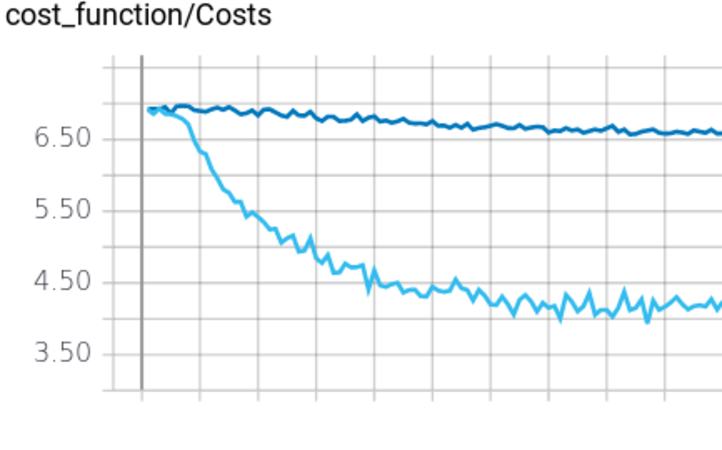
\includegraphics[width=\textwidth]{Kapitel/20Pretraining/Bilder/SGDvsADAMcost.pdf}
	\end{minipage}
	\hfill
	\begin{minipage}[b]{0.48\textwidth}		
		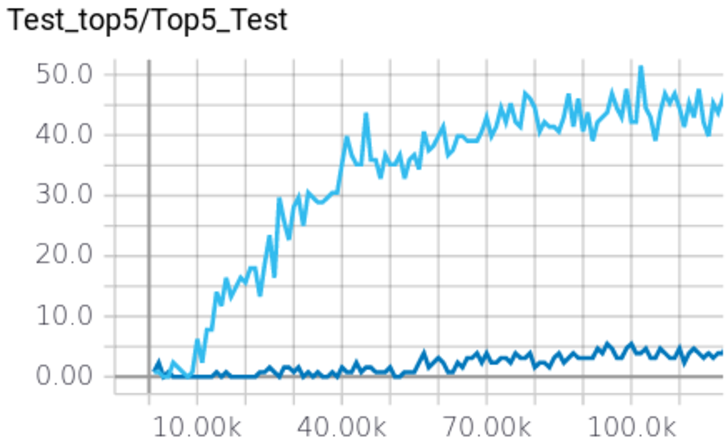
\includegraphics[width=\textwidth]{Kapitel/20Pretraining/Bilder/SGDvsADAMtop5.pdf}
	\end{minipage}
	\caption{Kosten und Top5-Test von vergleichbaren Tasks im Pretraining über einen beschränkten Zeitraum.
	links: [x-Achse=Zeit, y-Achse=Kosten]
	rechts: [x-Achse=Zeit, y-Achse=Top-5 Treffer in \%] 
	SGD=dunkelblau.
	ADAM=hellblau.}
	\label{img:SGDvsADAM}
\end{figure}
\subsection{Tests \& Resultate}
%Test Top 5 Pretraining
\begin{figure}	
	\centering
	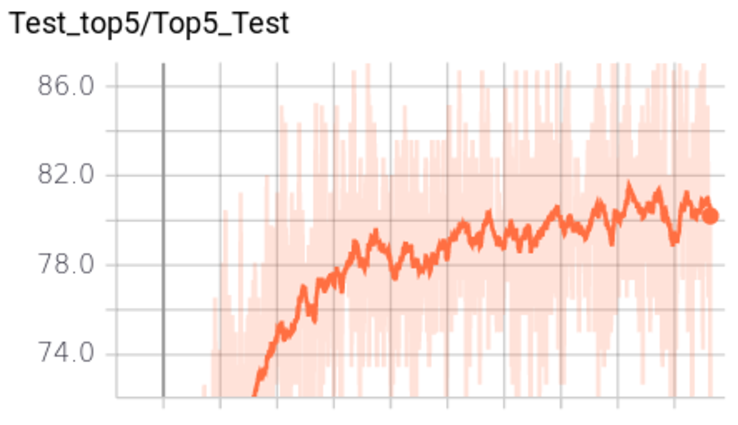
\includegraphics[width=.7\textwidth]{Kapitel/20Pretraining/Bilder/Test_top5.pdf}
	\caption{Test-Top5 nach 6 Tagen Lernzeit(x-Achse=Zeit, y-Achse=Top-5-Treffer in \%)}
	\label{img:test_top5}
\end{figure}   
Das Testen dieses Tasks war sehr einfach.
Es konnte einfach aus dem Outputvektor der Index des Elements mit dem Grössten Wert genommen und mit dem One-Hot-Index des Label-Vektors verglichen werden. 
Waren die beiden identisch, war die Vorhersage korrekt. 
Um das Resultat mit dem Resultat aus dem Yolo-Paper \cite{yolo} vergleichen zu können, wurde nicht nur der Index des höchsten Wertes im Output-Vektor verwendet, sondern gleich die Indexen der 5 höchsten Werte. 
Wie man in der Abbildung \ref{img:test_top5} wurde nach 6 Tagen Lernzeit im Top5-Test im Schnitt eine Treffsicherheit von rund 80\% erreicht.
Da im nach dem originalen Yolo-Paper \cite{yolo} eine Treffsicherheit von 88\% erreicht wurde, war das Resultat dieser Arbeit um rund 8\% schlechter.

Es gibt zwei unbestätigte Vermutungen, was der Grund für diese schlechtere Performance sein könnte: 
\begin{enumerate}
\item In dieser Arbeit wurden nur Grayscaleinformationen eines Bildes verwendet, während im originalen Yolo-Paper \cite{yolo} die volle Farbinformation mitverwendet wurde. Der Grund, weshalb grayscale verwendet wurde ist, dass wir für das spätere Training ebenfalls nur Grayscale-Bilder zur Verfügung hatten.
\item Um Aufwand einzusparen wurde in dieser Arbeit nicht auf dem Image-Net Validation-Set validiert, sondern ein Teil der Trainingsdaten zum validieren verwendet. Diese Daten fehlten entsprechend im Training, was ebenfalls eine Reduktion der Treffsicherheit zur Folge gehabt haben könnte. 
\end{enumerate}
Diesen Vermutungen wurde während dieser Arbeit nicht nachgegangen, da mit 80\% Genauigkeit im Top5-Test erst einmal vorwärts gearbeitet werden konnte. 



\subsection{Gewichte}
Während dem Training wurden die Gewichte erst einmal regelmässig als Tensorflow-Gewichte-Dateien abgespeichert.
Um jedoch später möglichst flexibel zu sein wurden die besten Gewichte zusätzlich noch als Python-Objekte abgespeichert.
Dies geschah aus dem Grund, dass es zwischenzeitlich Probleme gab vortrainierte Gewichte direkt ins echte Training einzulesen, wenn man nicht genau dieselbe Architektur hatte wie im Pretraining, was offensichtlich der Fall war (Siehe Abbildung \ref{tbl:pretraining_Architektur} \& \ref{tbl:yolo_architektur}).
Es gäbe zwar Tricks, wie man einen Graph aufsplitten und so die Gewichte vom Pretraining im Training verwenden könnte. 
Dieser Ansatz wurde aber nicht weiter verfolgt, weil es einerseits mit den Pythongewichten gut funktioniert hatte und andererseits, weil der Speicher der GPU's beim Training schon voll war und die Gewichte des Pretraining-Astes nicht auch noch Platz gehabt hätten.

\subsection{Fazit}
Sobald man Tensorflow grundsätzlich verstanden hat, ist das bauen einer Klassifizierungs-Architektur eigentlich sehr einfach. 
Man muss dafür nicht einmal unbedingt die Theorie hinter dem Deeplearning verstanden haben, sondern muss einfach wissen, welche Bausteine \grqq{}man\grqq{} nimmt und wie diese angeordnet werden müssen.
Weil für das Training in einer ersten Phase entschieden wurde, dass für Gewichte und Knoten Float16 verwendet werden soll (siehe Kapitel \ref{chapter:Architekturaubau}), musste dies entsprechend auch im Pretraining so gemacht werden. 
Aus diesem Grund gab es auch im Pretraining einige Probleme mit nicht direkt erklärbaren Effekten (Abbildung \ref{img:overflow_pretraining}).
Es gab Vermutungen, dass es sich bei diesen Problemen um Overflow-Probleme gehandelt hatte.
Seit alles auf Float32(Standard in Tensorflow) umgestellt wurde, gab es entsprechend keinerlei solche Probleme mehr.
Dementsprechend ist die Empfehlung in Tensorflow was die Datentypen angeht, möglichst nicht vom Standard abzuweichen, auch wenn dies Einfluss auf die Architektur und andere wichtige Punkte nehmen kann.
\todo[inline,size=\Large]{Hier überprüfen, ob dieses Bild und der Abschnitt nicht allzu redundant mit dem Kapitel Training sind....}
\begin{figure}
	\centering
	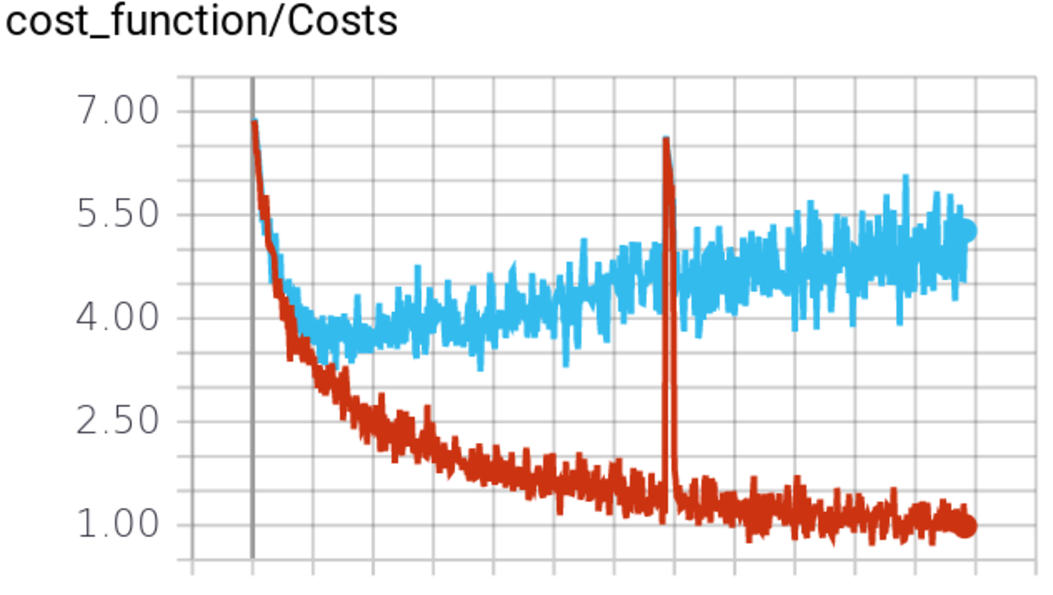
\includegraphics[width=.7\textwidth]{Kapitel/20Pretraining/Bilder/Overflow.pdf}
	\caption{Effekte in Training(Weinrot) und Validierung(Hellblau) mit Float16. x-Achse=Zeit, y-Achse=Kosten}
	\label{img:overflow_pretraining}
\end{figure}  
 